\documentclass[10pt, a4paper]{article}
\usepackage[utf8x]{inputenc}            % Acentos, ñ, etc.
\usepackage{graphicx}                   % Gráficos
\usepackage[spanish]{babel}             % Macros en español
\usepackage{caratula}                   % Carátula
\usepackage{geometry}                   % Márgenes
\usepackage{listings}
\begin{document}

\subsection{¿Cuál es el espacio de estados?}

Cada configuracion posible del tablero es un estado, es decir guardamos para cada posición del tablero si hay una ficha y de que jugador. Muchos de esos estados son inalcanzables, ya que toda ficha debe estar inmediatamente por encima de otra ficha. Tampoco consideramos estados en los que hay cuatro fichas alineadas (ya sea de forma vertical, horizontal o diagonal). 
Cada accion se corresponde con insertar una ficha en alguna de las columnas. La ficha será asignada a la fila inmediatamente superior a la fila donde estaba la ficha más arriba en la misma columna.

Las recompensas a las acciones tomadas se otorgan después de que juegue el rival, excepto en los casos en los que la partida finaliza.


En este trabajo observamos cuanto aprenden los modelos a partir de la cantidad de victorias que tienen contra otros modelos.
Hay muchos parámetros en el modelo que se podían modificar para variar:
\begin{itemize}
	\item $\epsilon$
	\item $\gamma$
	\item $\alpha$
	\item Recompensa por ganar el partido
	\item Recompensa por perder el partido
	\item Recompensa por empatar el partido
	\item Recompensa por un nuevo turno
	\item La cantidad de iteraciones que se entreno

\end{itemize}



¿Cuál es el espacio de estados?, ¿cuán rápido se puede explorar?, ¿cómo cambia la inicialización de Q con respecto a la velocidad de aprendizaje?, ¿qué importancia tiene la temperatura y la velocidad con que se enfría el sistema si se decide usar la distribution Boltzmann?, ¿qué efecto tiene cambiar la tasa de aprendizaje?, etc.

\section{Experimentación}

\subsection{Experimentación Inicial}

Primero hicimos competir al QLP contra el jugador Random y contra otro QLP.

\newgeometry{left=1cm,right=1cm}
\begin{figure}[ht]
  \begin{minipage}[c]{1\textwidth}
	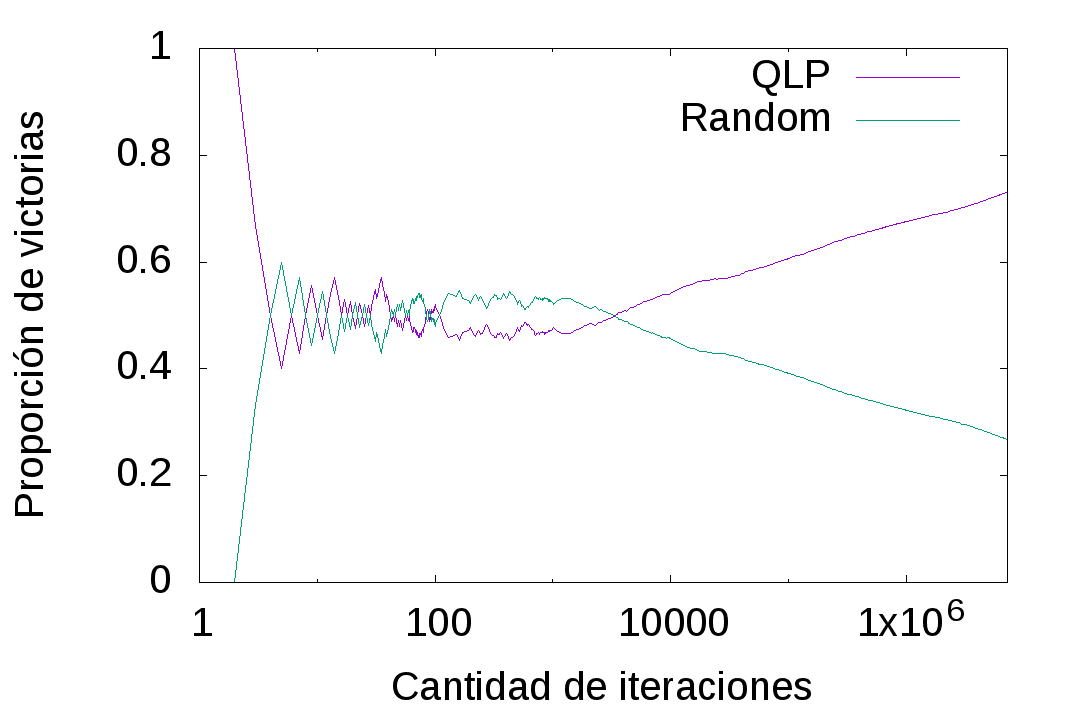
\includegraphics[scale=0.32]{Initial/QvR.png}
	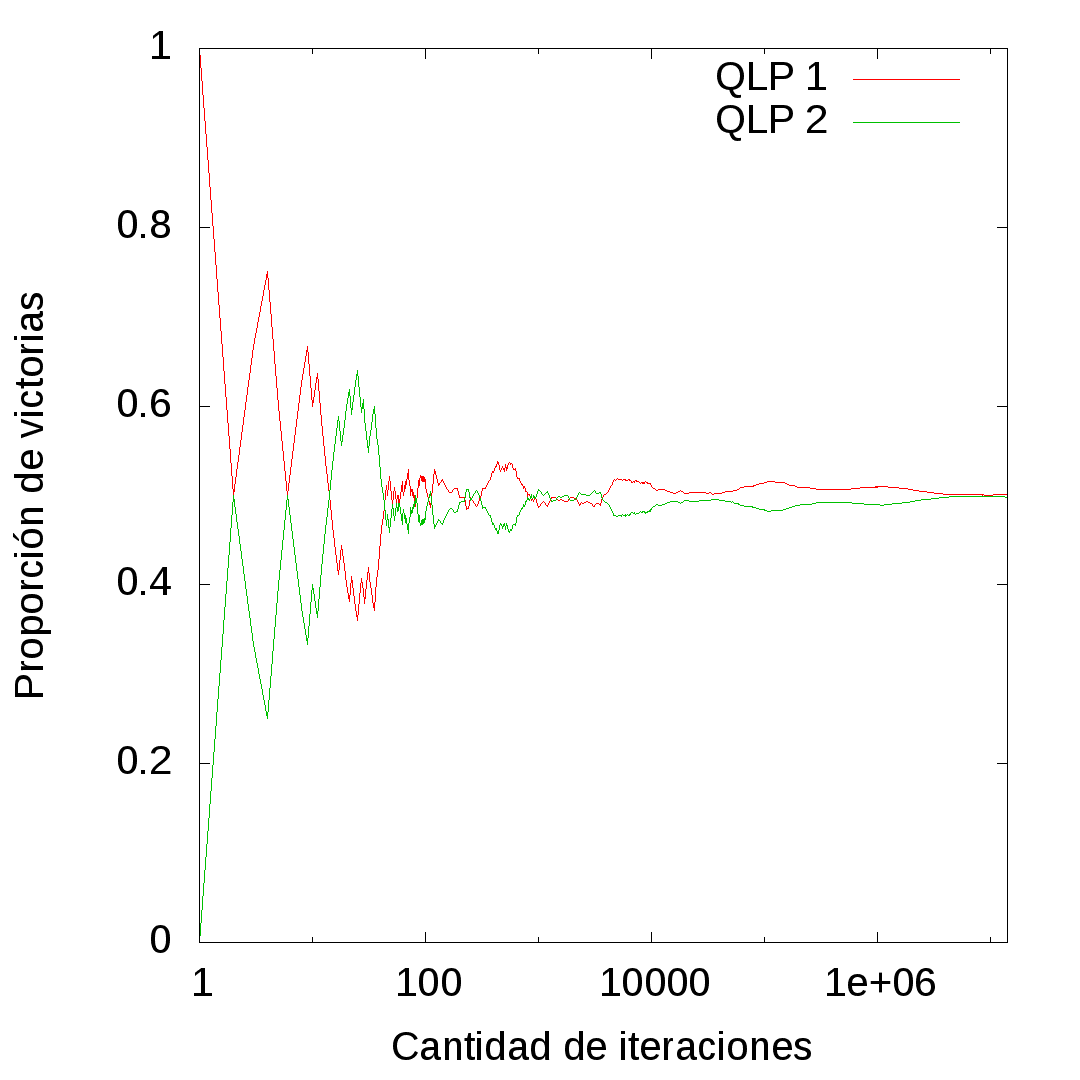
\includegraphics[scale=0.32]{Initial/QvQ.png}
  \end{minipage}
\end{figure}
\restoregeometry



\subsection{Ajuste de parámetros}

Experimentamos variando los parámetros $\alpha$, $\gamma$ y $\epsilon$ por separado, haciéndolo competir contra un jugador Random y contra un jugador con los parámetros por defecto ($\alpha=0.3,\gamma=0.9 y \epsilon=0.2$).
Cabe aclarar que mientras variamos un parámetro del modelo, los otros dos se fijan tambien en los valores por defecto ya mencionados.

\newgeometry{left=1cm,right=1cm}
\begin{figure}[ht]
 \centering
  \begin{minipage}[c]{1\textwidth}
	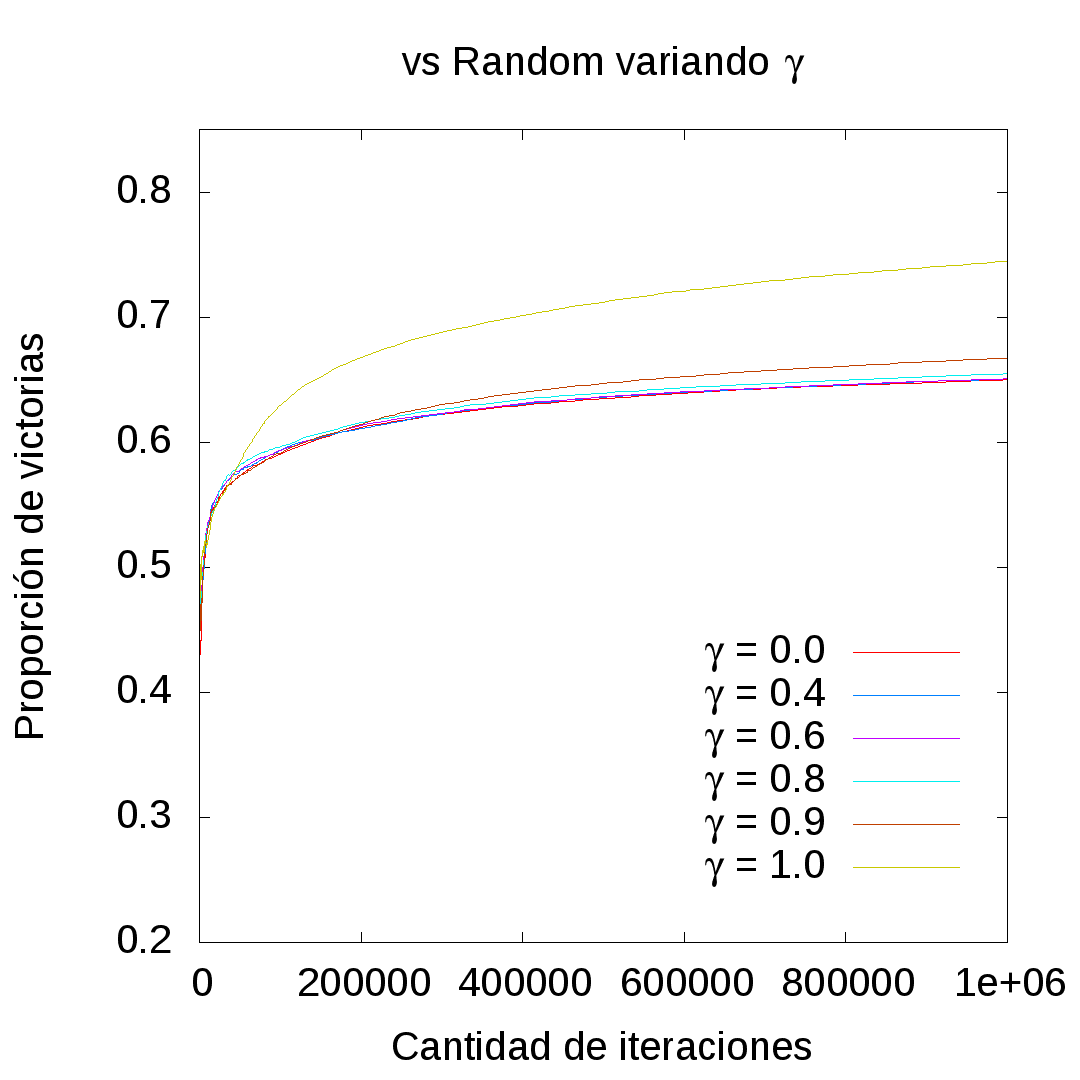
\includegraphics[scale=0.32]{GammaR.png}
	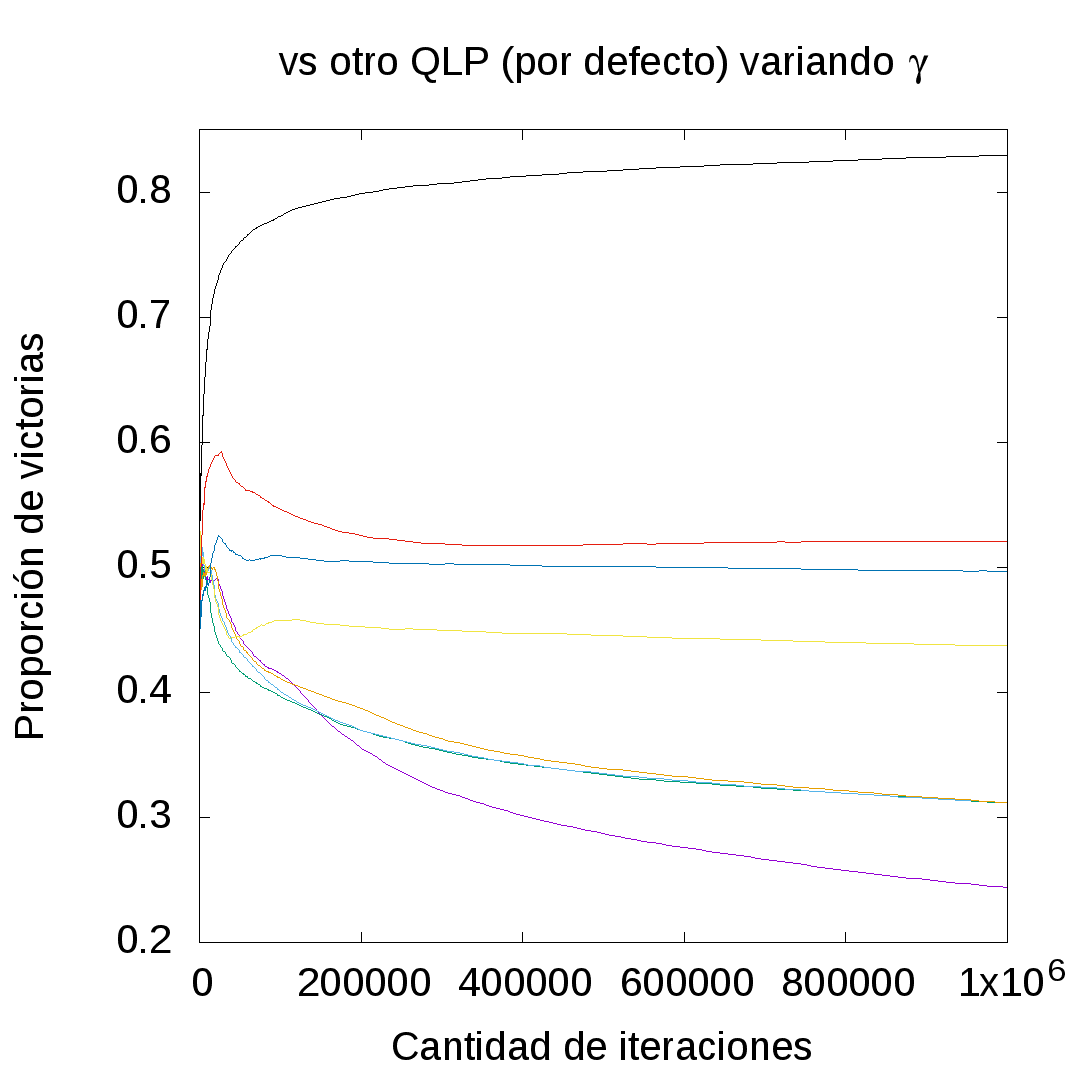
\includegraphics[scale=0.32]{GammaQ.png}
	Aquí observamos que el mejor valor que puede tomar $\gamma = 1$ ya que tiene mayor cantidad de victorias y tiene un aprendizaje más rápido en ambas competencias (vs un jugador random y vs otro jugador QLearner). 
  \end{minipage}
\end{figure}
\begin{figure}[ht]
  \begin{minipage}[c]{1\textwidth}
	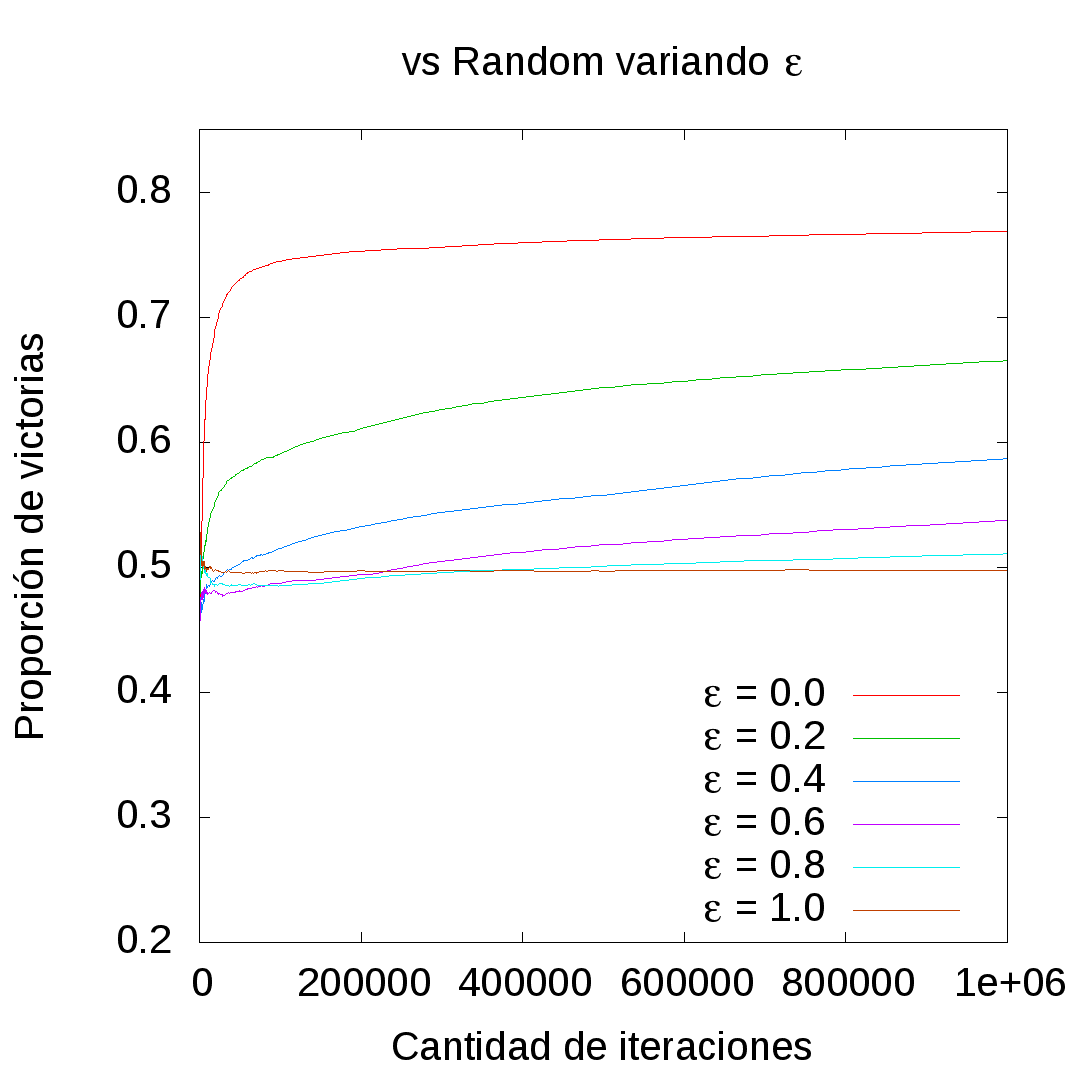
\includegraphics[scale=0.32]{EpsilonR.png}
	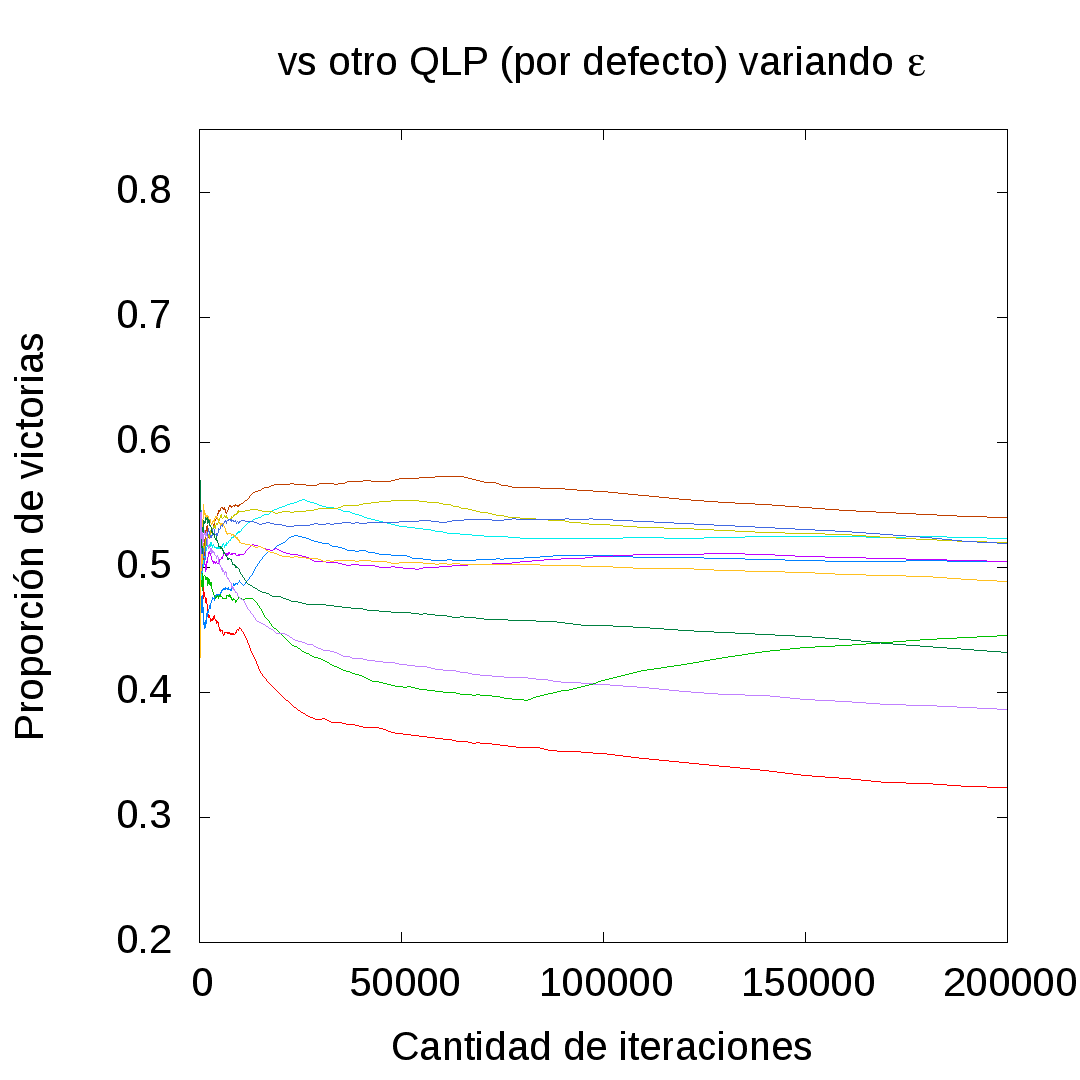
\includegraphics[scale=0.32]{EpsilonQ.png}
	En este caso, no  hay un claro valor óptimo. Sin embargo elegimos seguir con $\epsilon=0.2$ ya que en ambos casos termina segundo en cuanto a la cantidad de victorias después de un millón de iteraciones.
  \end{minipage}
\end{figure}
\begin{figure}[ht]
  \begin{minipage}[c]{1\textwidth}
	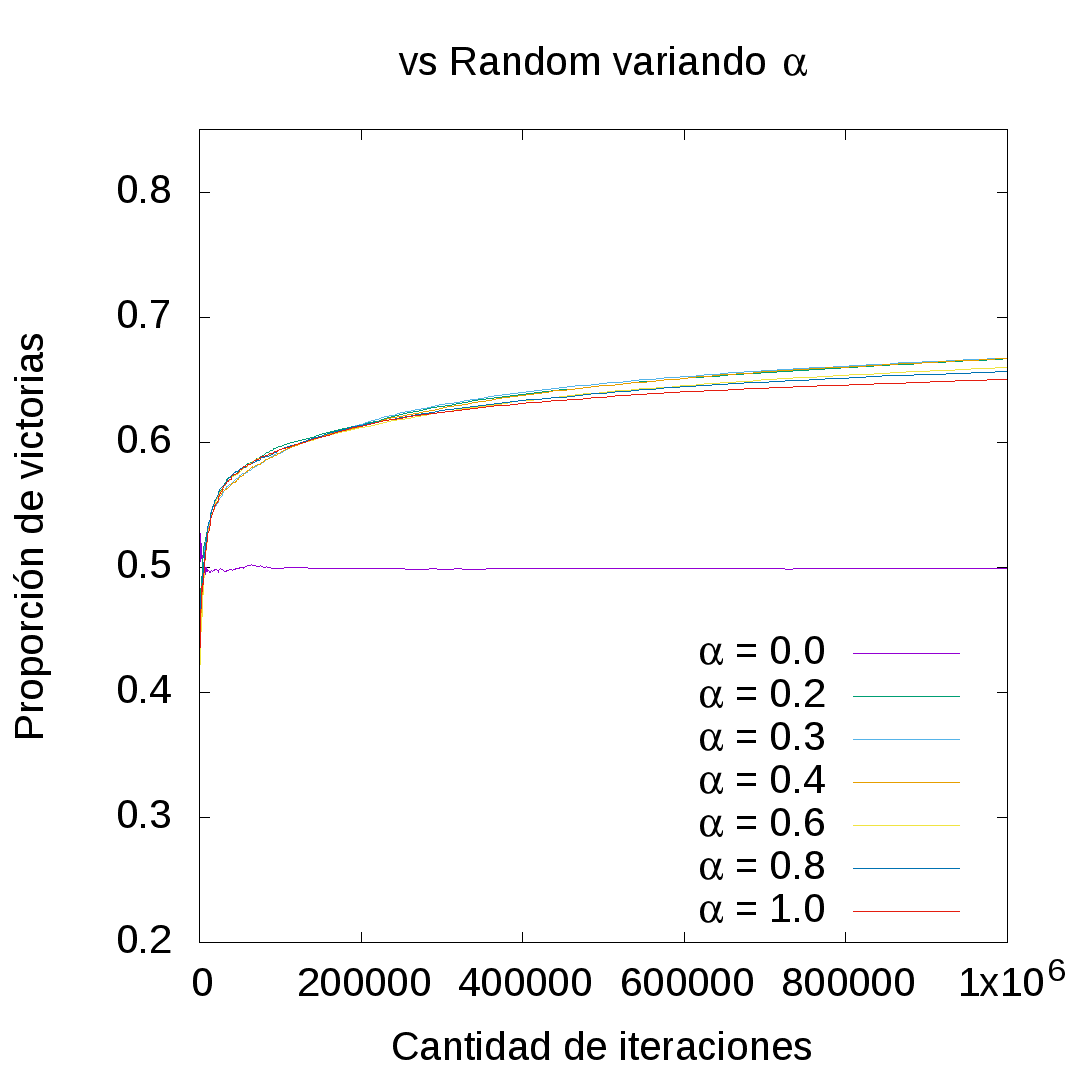
\includegraphics[scale=0.32]{AlphaR.png}
	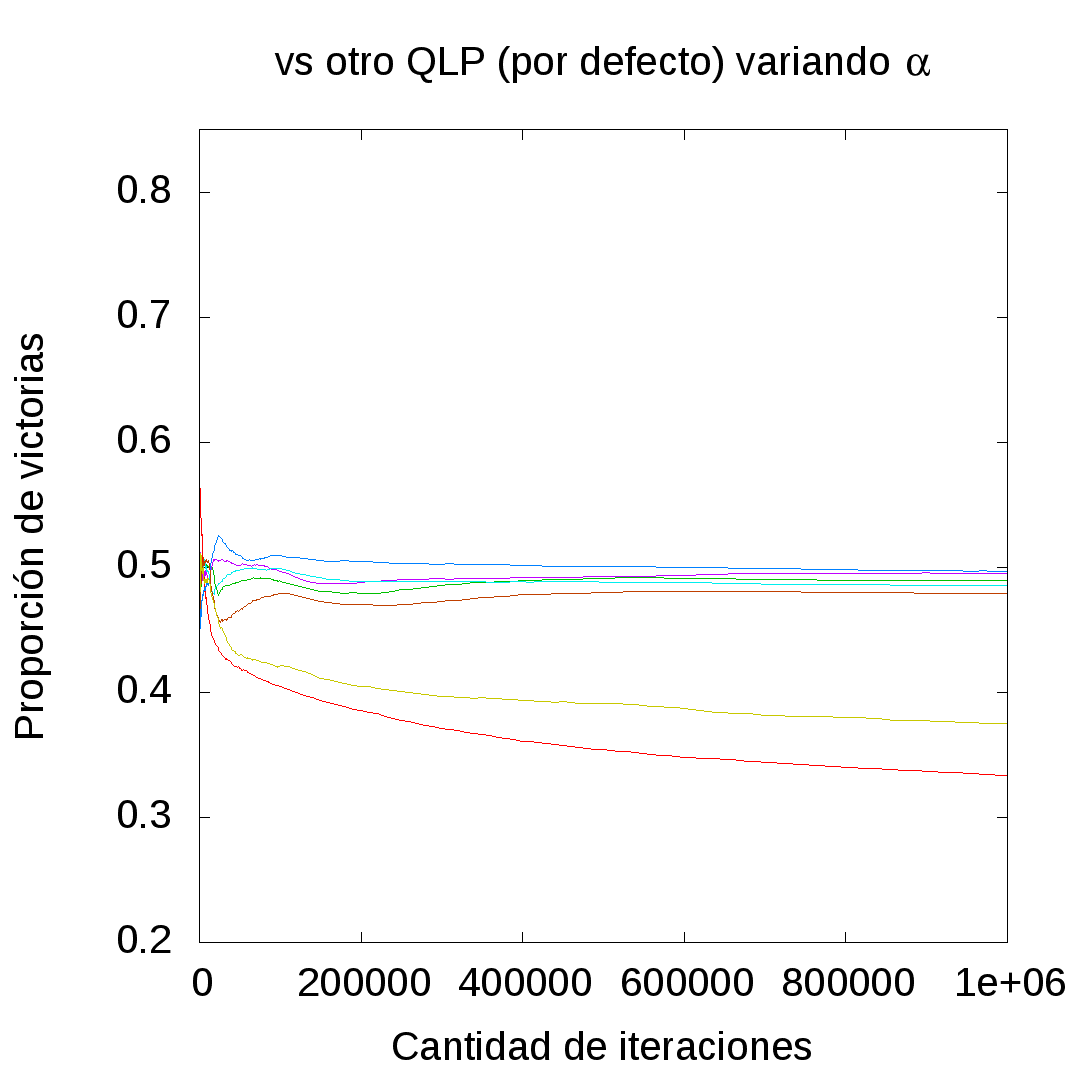
\includegraphics[scale=0.32]{AlphaQ.png}
	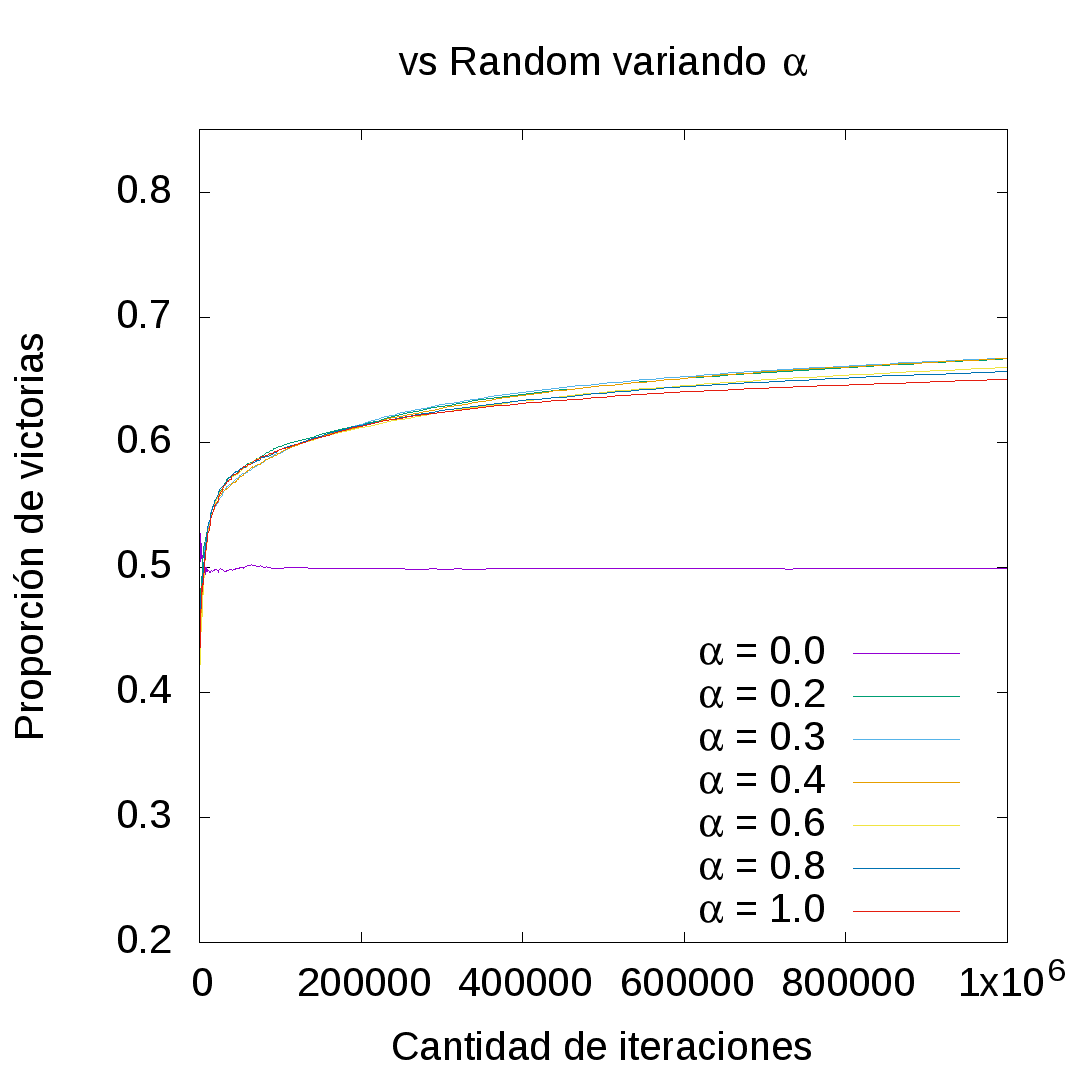
\includegraphics[trim=230mm 185mm 13mm 90mm, clip, scale=2.5]{AlphaR.png}
	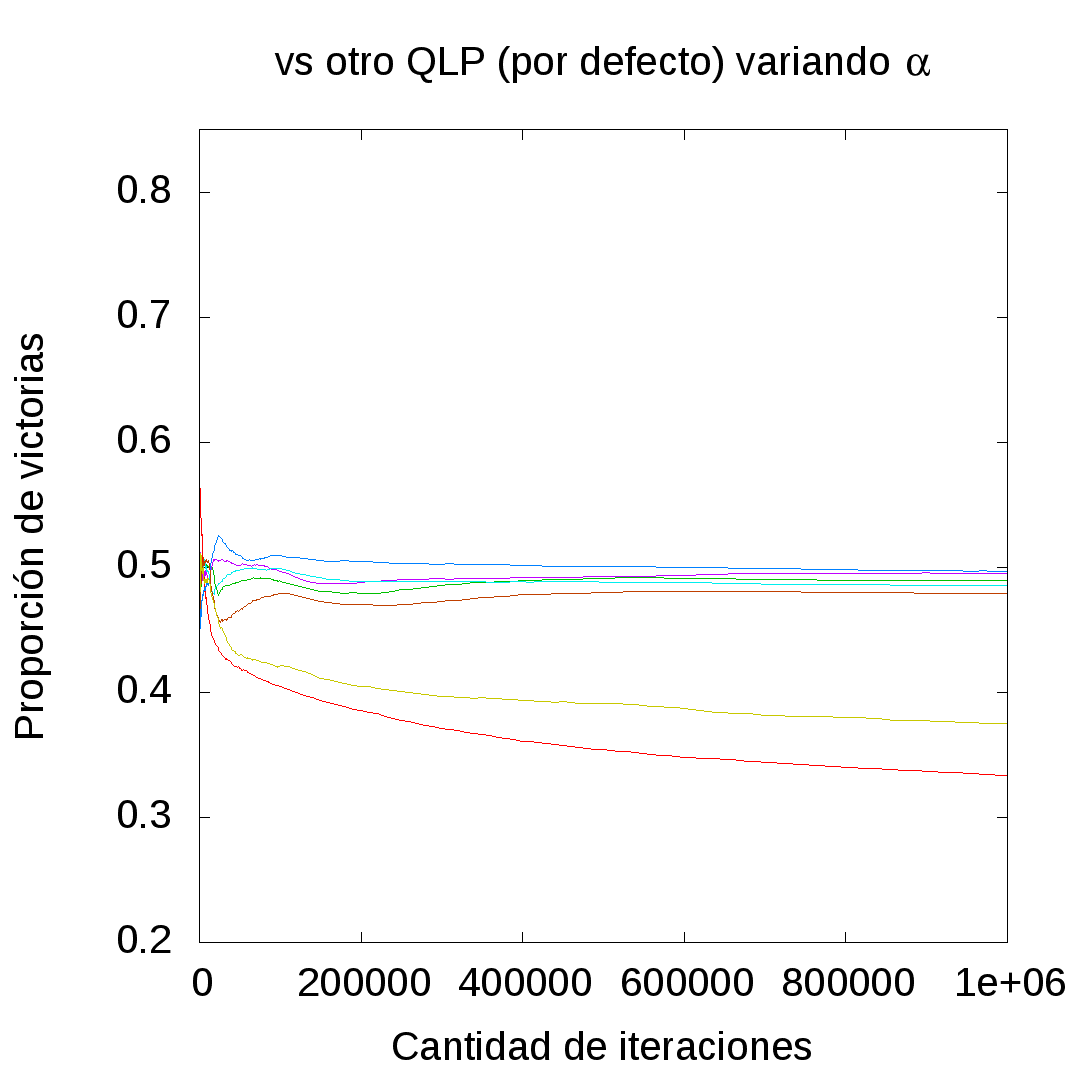
\includegraphics[trim=235mm 125mm 0mm 150mm, clip, scale=2.5]{AlphaQ.png}
	Variando $\alpha$ hay una diferencia sútil en los distintos modelos pero el mejor valor es $\alpha=0.3$. También se puede observar que con $\alpha=0$, el modelo se comporta como un jugador Random, algo esperable ya que es el caso en que no hay exploración.
  \end{minipage}
\end{figure}

\restoregeometry


\subsection{Experimentos con parámetros ajustados}

Explicacion de que llamamos competencia

\subsubsection{Caso 1(QQ vs QR)}

Grafico del entranmiento y grafico de torta/barra con la competencia Resultados

\subsubsection{Caso 2(QQR vs QRQ)}

Grafico del entranmiento y grafico de torta/barra con la competencia Resultados

\subsubsection{Caso 3(QQ vs QR vs QS)}

Explicacion de que es el S Grafico del entranmiento y grafico de torta/barra con la competencia Resultados


Ideas que no llegamos a hacer ???

Contar de la idea de implementar un minimax, pero que no lo pusimos en practica porque era infinito.

variando las recompensas?

q(vsRandom) vs q(vsQ) con epsilon 0, osea no siguen aprendiendo.


4x4 y ver si eso lleva a  mas empates
comparar si cambiamos ganancia de empate a 0.
¿juagada ganadora? Veamos si siempre empieza el jugador 1.






\section{Conclusiones}

\section{Como ejecutar el tp}



En el caso en los que los valores de $\alpha$, $\gamma$ y $\epsilon$ son por defecto:
\begin{lstlisting}
python fourInLine.py key1 key2 [iteraciones]  
\end{lstlisting}
donde key son los tipos de jugadores. Caso contrario: \\
\begin{lstlisting}
python fourInLine.py p key1 key2 a1 g1 e1 a2 g2 e2 rw rt rl rr save [iters]
\end{lstlisting}

\end{document}
